\documentclass{panikzettel}

\title{Panikzettel EMS}
\author{Kevin Conrads}

\usepackage{listings}
\lstset{basicstyle=\ttfamily\footnotesize,breaklines=true}

\newcommand\tab[1][1cm]{\hspace*{#1}}
\newcommand{\boxspace}{	\vspace{-\baselineskip}	}

\begin{document}

\maketitle

\tableofcontents

\section{Einleitung}
Dieser Panikzettel für das Fach ``Einführung in Management Science: Desgin und Analyse von Algorithmen'', gehalten im WS19/20 von Prof. Peis, ist ein freiwilliges Projekt, dass ich parallel zu meiner Tutortätigkeit in diesem Fach erstellt habe. Die Struktur folgt dabei in der Reihenfolge den Vorlesungsthemen, kann jedoch an sinnvollen Stellen davon abweichen.

Dieses Dokument hat \emph{nicht} zum Ziel, alleinige Ressource zum Lernen und Verstehen des Vorlesungsstoffes zu sein, sondern eine begleitende bzw. ergänzende Rolle zu den Materialien aus der Vorlesung und Übung einzunehmen. Trotz größter Sorgfalt können Fehler, die Inhalt, Form, Notation, etc. betreffen, nicht ausgeschlossen werden. Es liegt daher in der Verantwortung des/der Leser/Leserin, sich im Zweifel mit den betreffenden Lehrmaterialien der Vorlesung auseinanderzusetzen. Außerdem hafte ich nicht für falsche Antworten in z.B. der Klausur, aufgrund der Informationen in diesem Dokument getätigt wurden. 

Eltern haften für ihre Kinder.

\todo[inline]{Hinweis auf Mathelight, Notationshilfen, Übungsmaterialen, etc.}

\vspace{-0.5\baselineskip}
{\small{}
	\paragraph{Hinweis:}
	Das Latex-Template für diesen Panikzettel sowie das Konzept ``Panikzettel'' an sich sind übernommen bzw. angelehnt an das \href{https://git.rwth-aachen.de/philipp.schroer/panikzettel}{Panikzettel-Projekt}.

\section{Stabile Matchings}

\subsection{Das Stable Marriage Problem}

\begin{halfboxl}
	\vspace{-\baselineskip}
	\begin{defi}{Stable Marriage Problem}
	Das Stable Marriage Problem beschreibt, wie eine Menge von Männern und eine gleichgroße Menge von Frauen miteinander verlobt (\emph{gematched}) werden sollen, so das keiner einen Anreiz zu einem Seitensprung hat.\\
	
	\begin{itemize}
		\item Es gibt eine Menge an $n$ Männern und eine Menge an $n$ Frauen
		\item Jeder Mann listet die Frauen nach absteigender Präferenz
		\item Jede Frau listet die Männer nach absteigender Präferenz
		\item Gesucht ist ein Arrangement an $n$ Hochzeiten, das heißt ein \emph{perfektes Matching}
		\item Das Matching soll möglichst stabil sein: Keiner sollte einen Anreiz zu einem Seitensprung haben
	\end{itemize}
	\end{defi}
\end{halfboxl}%
\begin{halfboxr}
	 \vspace{-\baselineskip}
	Graph-Beispiel für das Stable Marriage Problem:\\
	
	\begin{center}
	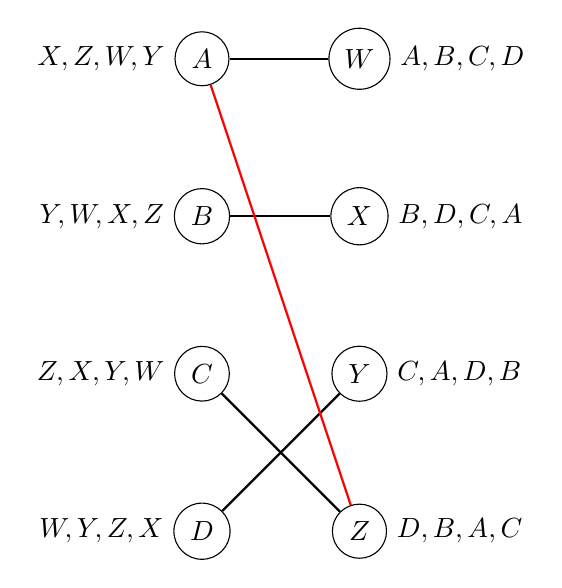
\begin{tikzpicture}
	\node[draw,circle,minimum size=5mm, label = left:{$X,Z,W,Y$}] (A) at (0,0) {$A$};
	\node[draw,circle,minimum size=5mm, label = left:{$Y,W,X,Z$}] (B) at (0,-2) {$B$};
	\node[draw,circle,minimum size=5mm, label = left:{$Z,X,Y,W$}] (C) at (0,-4) {$C$};
	\node[draw,circle,minimum size=5mm, label = left:{$W,Y,Z,X$}] (D) at (0,-6) {$D$};
	
	\node[draw,circle,minimum size=5mm, label = right:{$A,B,C,D$}] (W) at (2,0) {$W$};
	\node[draw,circle,minimum size=5mm, label = right:{$B,D,C,A$}] (X) at (2,-2) {$X$};
	\node[draw,circle,minimum size=5mm, label = right:{$C,A,D,B$}] (Y) at (2,-4) {$Y$};
	\node[draw,circle,minimum size=5mm, label = right:{$D,B,A,C$}] (Z) at (2,-6) {$Z$};
	%\foreach \X [count=\Y from 2] in {1, ..., 3}{
	%	\draw[-] (\X) -- (\Y);
	%}
	\draw[thick] (A) -- (W);
	\draw[thick] (B) -- (X);
	\draw[thick] (C) -- (Z);
	\draw[thick] (D) -- (Y);
	\draw[thick,red] (A) -- (Z);
	\end{tikzpicture}
	
	Hier liegt ein instabiles Matching vor: $\{A,Z\}$ sind unzufrieden mit der Partnerwahl; sie finden sich gegenseitig besser als ihre jetzigen Partner und hätten damit Anlass für einen Seitensprung.
	\end{center}
\end{halfboxr}

%\vspace{0.5cm}

\begin{halfboxl}
	\vspace{-\baselineskip}
	\begin{defi}{Matchings in Graphen}
	Sei $G = (V,E)$ ein ungerichteter Graph\\
	
	\begin{itemize}
	\item Eine Teilmenge $M$ der Kanten wird Matching gennant, wenn keine zwei Kanten in $M$ einen gemeinsamen Endknoten haben.
	
	\item Die Kardinalität $|M|$ (Anzahl der Kanten in $M$) eines Matchings $M$ ist nie größer als $\frac{|V|}{2}$
	
	\item Ein Matching $M$ mit $|M| = \frac{|V|}{2}$ heißt \emph{perfekt}
	
	\end{itemize}
	\end{defi}
\end{halfboxl}%
\begin{halfboxr}
	\vspace{-\baselineskip}
	\begin{defi}{Bipartite Graphen}
	Ein ungerichteter Graph $G = (V,E)$ heißt \emph{bipartit}, wenn sich die Knotenmenge $V$ so in zwei Hälften aufteilen lässt, dass\\
	
	\begin{itemize}
		\item $V = L \cup R$ (jeder Knoten ist entweder in $L$ oder in $R$),
		\item $L \cap R = \emptyset$ (kein Knoten liegt in beiden Mengen) und 
		\item das jede Kante einen Endknoten in $L$ und einen in $R$ besitzt.
	\end{itemize}
	\end{defi}
\end{halfboxr}

\begin{defi}{Blockierende Kante und Stabiles Matching}
	Eine Kante ${u,v}$ heißt \emph{blockierend} (für ein Matching $M$), wenn der Knoten $u$ den Knoten $v$ gegenüber seinem jetzigen Partner präferiert und umgekehrt.
	
	Ein Matching $M$ ist \emph{stabil}, wenn es keine blockierende Kante im Graphen gibt.
	
	\textit{(Im Beispiel Graph oben ist die rot gezeichnete Kante $\{A,Z\}$ eine blockierende Kante für das Matching.)}
\end{defi}

Hier sollte deutlich werden, dass das Stable Marriage Problem äquivalent zum Stable Matching Problem in bipartiten Graphen ist.

Das ``Reduzieren'' von Problem aus der Realität auf Probleme z.B. der Graphentheorie ist eine weit verbreitete Technik. Man folgt der Idee: Wenn man einen Algorithmus A hat, der ein (abstraktes) (Graphen-)Problem X löst, und ein reales Problem Y auf das Problem X reduzierbar (oder äquivalent) ist, dann kann man auch Problem Y mit dem Algorithmus A lösen.

\subsection{Exkurs: Stable Roommate Problem}

\begin{halfboxl}
	\vspace{-\baselineskip}
	\begin{defi}{Stable Roommate Problem}
		Das Stable Roommate Problem beschreibt, wie eine Menge von Personen anhand von Präferenzen in Paare aufgeteilt werden kann, sodass das resultierende Matching stabil ist.\\
		
		\begin{itemize}
			\item Gegeben: $2n$ Personen; jede Person sortiert die anderen $2n-1$ Personen in einer Präferenzlist
			\item Gesucht: Eine Aufteilung der $2n$ Personen in $n$ Paare, so dass das entsprechende (perfekte) Matching stabil ist.
		\end{itemize}
	
		Beim Stable Roommate Problem gibt es nicht immer ein stabiles perfektes Matching (siehe Beispiel rechts).
	\end{defi}
\end{halfboxl}%
\begin{halfboxr}
	\vspace{-\baselineskip}	
	\begin{center}
		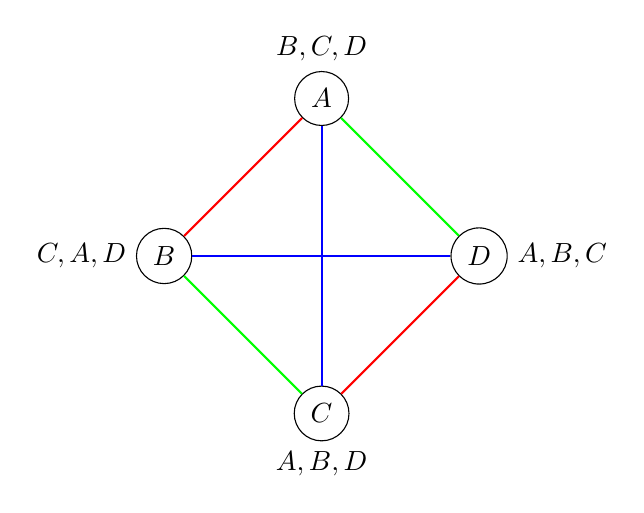
\begin{tikzpicture}
		\node[draw,circle,minimum size=5mm, label = above:{$B,C,D$}] (A) at (2,0) {$A$};
		\node[draw,circle,minimum size=5mm, label = left:{$C,A,D$}] (B) at (0,-2) {$B$};
		\node[draw,circle,minimum size=5mm, label = below:{$A,B,D$}] (C) at (2,-4) {$C$};
		\node[draw,circle,minimum size=5mm, label = right:{$A,B,C$}] (D) at (4,-2) {$D$};
		
		%\foreach \X [count=\Y from 2] in {1, ..., 3}{
		%	\draw[-] (\X) -- (\Y);
		%}
		\draw[thick,red] (A) -- (B);
		\draw[thick,green] (B) -- (C);
		\draw[thick,red] (C) -- (D);
		\draw[thick,green] (D) -- (A);
		\draw[thick,blue] (A) -- (C);
		\draw[thick,blue] (B) -- (D);
		\end{tikzpicture}
		
		Alle Möglichkeiten an Matchings (rot, blau, grün) sind nicht stabil.
	\end{center}
\end{halfboxr}

\subsection{Algorithmen zum Lösen des Stable Marriage Problems}

Es gibt zwei Algorithmen, die hier betrachtet werden: Die Seitensprung-Dynamik und Gale-Shapley-Algorithmus.

\subsubsection{Seitensprung-Dynamik}
\begin{algo}
	\textbf{Eingabe:} Beliebiges Matching $M$
	
	\textbf{Ausgabe:} Stabiles, perfektes Matching $M^*$.
	\tcblower
	
	\textbf{WHILE} (unzufriedenes Paar $\{m,w\}$ existiert)

	\tab Ersetze die Matchingkanten $\{m,w'\}$ und $\{m',w\}$ durch $\{m,w\}$ und $\{m',w'\}$
   
	\textbf{RETURN} $M^*$
	
\end{algo}

Folgender Graph zeigt eine Iteration innerhalb der \textbf{WHILE} Schleife:

\begin{halfboxl}
	\vspace{-\baselineskip}	
	\begin{center}
		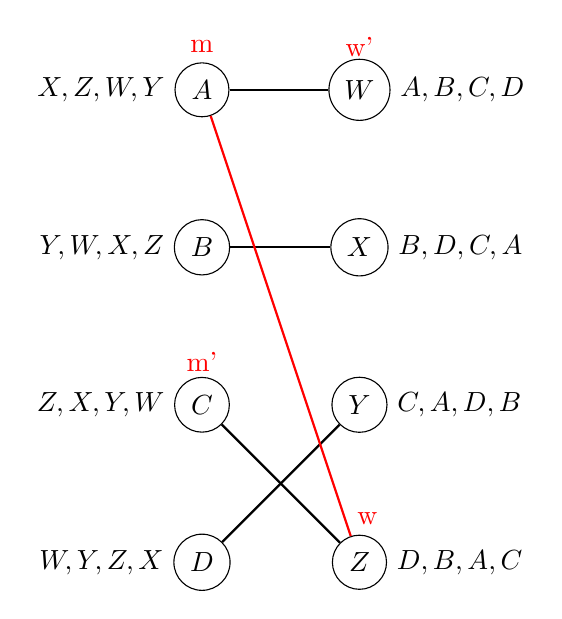
\begin{tikzpicture}
		\node[draw,circle,minimum size=5mm, label = left:{$X,Z,W,Y$}] (A) at (0,0) {$A$};
		\node[draw,circle,minimum size=5mm, label = left:{$Y,W,X,Z$}] (B) at (0,-2) {$B$};
		\node[draw,circle,minimum size=5mm, label = left:{$Z,X,Y,W$}] (C) at (0,-4) {$C$};
		\node[draw,circle,minimum size=5mm, label = left:{$W,Y,Z,X$}] (D) at (0,-6) {$D$};
		
		\node[draw,circle,minimum size=5mm, label = right:{$A,B,C,D$}] (W) at (2,0) {$W$};
		\node[draw,circle,minimum size=5mm, label = right:{$B,D,C,A$}] (X) at (2,-2) {$X$};
		\node[draw,circle,minimum size=5mm, label = right:{$C,A,D,B$}] (Y) at (2,-4) {$Y$};
		\node[draw,circle,minimum size=5mm, label = right:{$D,B,A,C$}] (Z) at (2,-6) {$Z$};
		\node[red] (m) at (0,0.55) {m};
		\node[red] (w) at (2.1,-5.45) {w};
		\node[red] (m2) at (0,-3.45) {m'};
		\node[red] (w2) at (2,0.55) {w'};
		
		%\foreach \X [count=\Y from 2] in {1, ..., 3}{
		%	\draw[-] (\X) -- (\Y);
		%}
		\draw[thick] (A) -- (W);
		\draw[thick] (B) -- (X);
		\draw[thick] (C) -- (Z);
		\draw[thick] (D) -- (Y);
		\draw[thick,red] (A) -- (Z);
		\end{tikzpicture}
	\end{center}

	$\{A,Z\}$ sind unzufrieden. Löse Verbindung $\{A,W\}$ und $\{C,Z\}$ auf und ...
\end{halfboxl}%
\begin{halfboxr}
	\vspace{-\baselineskip}	
	\begin{center}
		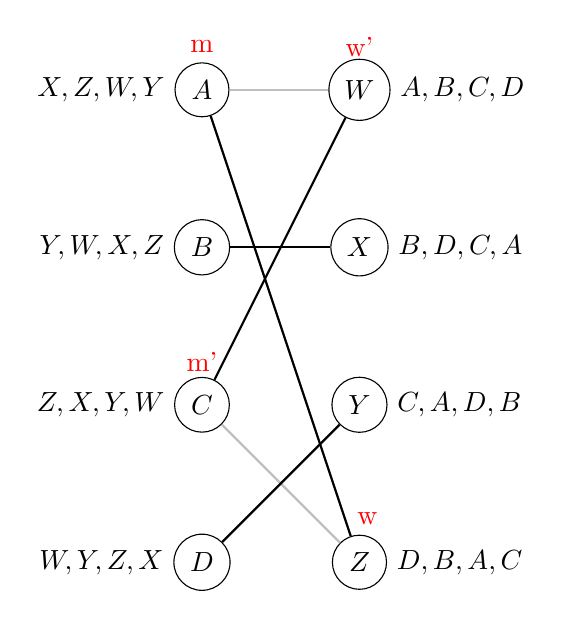
\begin{tikzpicture}
		\node[draw,circle,minimum size=5mm, label = left:{$X,Z,W,Y$}] (A) at (0,0) {$A$};
		\node[draw,circle,minimum size=5mm, label = left:{$Y,W,X,Z$}] (B) at (0,-2) {$B$};
		\node[draw,circle,minimum size=5mm, label = left:{$Z,X,Y,W$}] (C) at (0,-4) {$C$};
		\node[draw,circle,minimum size=5mm, label = left:{$W,Y,Z,X$}] (D) at (0,-6) {$D$};
		
		\node[draw,circle,minimum size=5mm, label = right:{$A,B,C,D$}] (W) at (2,0) {$W$};
		\node[draw,circle,minimum size=5mm, label = right:{$B,D,C,A$}] (X) at (2,-2) {$X$};
		\node[draw,circle,minimum size=5mm, label = right:{$C,A,D,B$}] (Y) at (2,-4) {$Y$};
		\node[draw,circle,minimum size=5mm, label = right:{$D,B,A,C$}] (Z) at (2,-6) {$Z$};
		
		\node[red] (m) at (0,0.55) {m};
		\node[red] (w) at (2.1,-5.45) {w};
		\node[red] (m2) at (0,-3.45) {m'};
		\node[red] (w2) at (2,0.55) {w'};
		
		%\foreach \X [count=\Y from 2] in {1, ..., 3}{
		%	\draw[-] (\X) -- (\Y);
		%}
		\draw[thick, lightgray] (A) -- (W);
		\draw[thick] (B) -- (X);
		\draw[thick,lightgray] (C) -- (Z);
		\draw[thick] (D) -- (Y);
		\draw[thick] (A) -- (Z);
		\draw[thick] (C) -- (W);
		\end{tikzpicture}
	\end{center}
	verbinde $\{A,Z\}$ und $\{C,W\}$. Die aufgelösten Kanten sind hier grau gefärbt.
\end{halfboxr}

\todo[inline]{Seitensprung-Dynamik Beispiel weglassen, aber dafür eins bei Gale-Shapley machen?}

\begin{theo}{Korrektheit der Seitensprung-Dynamik}
	Die Seitensprung-Dynamik terminiert nicht für jede Eingabe. Das heißt es wird nicht für alle Eingaben ein stabiles Matching gefunden. (Wenn man das Beispiel oben weiterführt, landet man irgendwann wieder an der Ausgangsposition).
\end{theo}

\subsubsection{Gale-Shapley Algorithmus}

Es gibt jedoch einen Algorithmus, der stets ein stabiles Matching findet:

\begin{algo}{Gale-Shapley}
	\textbf{Eingabe:} Ein bipartiter Graph $G$ mit einer Präferenzliste an jedem Knoten
	
	\textbf{Ausgabe:} Stabiles, perfektes Matching $M^*$.
	\tcblower
	
	Zu Beginn sind alle Männer und Frauen ungematched
	
	\textbf{WHILE} (es noch einen freien Mann gibt, der noch nicht allen Frauen einen Antrag gemacht hat)
	
	\tab Wähle einen solchen freien Mann $M$
	
	\tab Lasse diesen der besten Frau $w$ auf seiner Liste einen Antrag machen
	
	\tab \textbf{IF} (Frau $w$ ist noch frei)
	
	\tab\tab Verlobe $m$ und $w$
	
	\tab \textbf{ELSE} 
	
	\tab\tab  \textbf{IF} ($w$ findet $m$ besser als ihren aktuellen Verlobten $m'$)
	
	\tab\tab\tab Hebe die Verlobung von $w'$ und $m'$ auf
	
	\tab\tab\tab Verlobe $m$ und $w$
	
	\tab\tab\tab Streiche $w'$ von der Liste von $m'$
	
	\tab\tab \textbf{ELSE}
	
	\tab\tab\tab Streiche $w$ von der Liste von $m$
	
	Verheirate alle verlobten Paare
	
	\textbf{RETURN} das resultierende Matching $M^*$ von verheirateten Paaren
\end{algo}

Man beachte, dass ein Mann $m$ nur dann mit einer Frau $w$ verlobt wird, wenn entweder $w$ noch keinen Partner hat, oder wenn $w$ denn Mann $m$ besser als ihren bisherigen Verlobten $m'$ findet. Im Umkehrschluss bedeutet dies, das ein bereits verlobter Mann $m'$ seine Verlobte dadurch verlieren kann und wieder in die Liste der Männer hinzugefügt wird, die noch nicht allen Frauen einen Antrag gemacht hat. 

Ein perfektes Matching ist stabil, wenn entweder 
\begin{itemize}
	\item jeder Mann seine erste Wahl zur Partnerin hat, oder
	\item jede Frau ihre erste Wahl als Partner hat,
\end{itemize}
da so niemand den Anreiz zu einem Seitensprung hätte (dieser Fall tritt jedoch selten ein). Für Gale-Shapley gilt unabhängig davon: \todo{In einen Satz-Block packen}

\begin{theo}{Korrektheit von Gale-Shapley}
	Gale-Shapley berechnet stets ein stabiles perfektes Matching. 
	
	Der Algorithmus hat eine Laufzeit von $\mathcal{O}(n^2)$, wobei $n$ der Anzahl der Männer bzw. der Frauen entspricht.
\end{theo}

Unter Umständen kann es mehrere stabile Matchings in einem Graphen geben, daher stellt sich die Frage, welches Gale-Shapley findet. Man stellt zunächst fest, dass Gale-Shapley die Männer bevorzugt, da diese aktiv auswählen und die Frauen nur passiv abwarten. 

\begin{thirdboxl}
	\vspace{-\baselineskip}	
	\begin{defi}{Zulässige Partnerin}
		Eine Frau $w$ ist eine \emph{zulässige Partnerin} von Mann $m$, wenn es ein stabiles perfektes Matching gibt, bei dem $m$ und $w$ ein Paar bilden.
	\end{defi}

	\begin{defi}{Mann-optimal}
		Ein Matching wird \emph{Mann-optimal} genannt, wenn jeder Mann mit seiner bevorzugten zulässigen Partnerin zusammen ist
	\end{defi}
\end{thirdboxl}%
\begin{thirdboxm}
	\vspace{0.7cm}	
	\begin{center}
		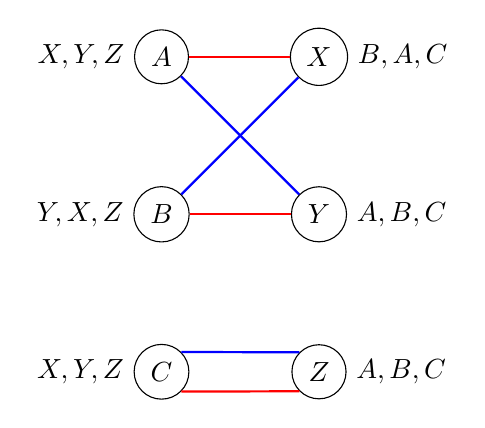
\begin{tikzpicture}
		\node[draw,circle,minimum size=5mm, label = left:{$X,Y,Z$}] (A) at (0,0) {$A$};
		\node[draw,circle,minimum size=5mm, label = left:{$Y,X,Z$}] (B) at (0,-2) {$B$};
		\node[draw,circle,minimum size=5mm, label = left:{$X,Y,Z$}] (C) at (0,-4) {$C$};
	
		\node[draw,circle,minimum size=5mm, label = right:{$B,A,C$}] (X) at (2,0) {$X$};
		\node[draw,circle,minimum size=5mm, label = right:{$A,B,C$}] (Y) at (2,-2) {$Y$};
		\node[draw,circle,minimum size=5mm, label = right:{$A,B,C$}] (Z) at (2,-4) {$Z$};
		
		\draw[thick,red] (A) -- (X);
		\draw[thick,red] (B) -- (Y);
		\draw[thick,red] (C.315) -- (Z.225);
		\draw[thick,blue] (A) -- (Y);
		\draw[thick,blue] (B) -- (X);
		\draw[thick,blue] (C.45) -- (Z.135);
		\end{tikzpicture}
	\end{center}
\end{thirdboxm}%
\begin{thirdboxr}
	\vspace{1.5cm}	
	\begin{itemize}
		\item $X$ und $Y$ sind zulässige Partnerinnen von $A$
		\item $X$ und $Y$ sind zulässige Partnerinnen von $B$
		\item nur $Z$ ist zulässige Partnerin von $C$. Jedes perfekte stabile Matching muss deshalb die Kante $\{C,Z\}$ enthalten
	\end{itemize}
\end{thirdboxr}

\begin{theo}{Gale-Shapley und Matchings}
	\begin{itemize}
		\item Mann-optimale Matchings sind perfekt und stabil.
		\item Gale-Shapley liefert stets ein Mann-optimales Matching.
		\item Gale-Shapley weist jeder Frau den für sie schlechtesten zulässigen Partner zu
	\end{itemize}

\end{theo}

\subsection{Kontext des Stable Marriage Problems: College Admission}

\begin{halfboxl}
	\vspace{-\baselineskip}
	\begin{defi}{College Admission Problem}
		Es gibt Studierende und Universitäten mit jeweiligen Präferenzen, die einander zugeteilt werden sollen.\\
		
		\begin{itemize}
			\item Studierende bzw. Universitäten können als inakzeptabel deklariert werden
			\item Es gibt nicht unbedingt gleich viele Studierende wie Unis
			\item Jede Uni hat eine Quote, die die maximale Anzahl zugewiesener Studis festlegt
		\end{itemize}
	
	Eine Zuweisung (hier spricht man nicht mehr von Matching, wie es oben definert wurde) ist zulässig, wenn jeder Studi einer akzeptable Uni zugewiesen wurde und jeder Uni nur akzeptable Studis zugewiesen wurde. Auch hier kann es analog "blockierende" Kanten geben.
	\end{defi}
\end{halfboxl}%
\begin{halfboxr}
	\vspace{-\baselineskip}
	Graph-Beispiel für das College Admission Problem:\\
	
	\begin{center}
		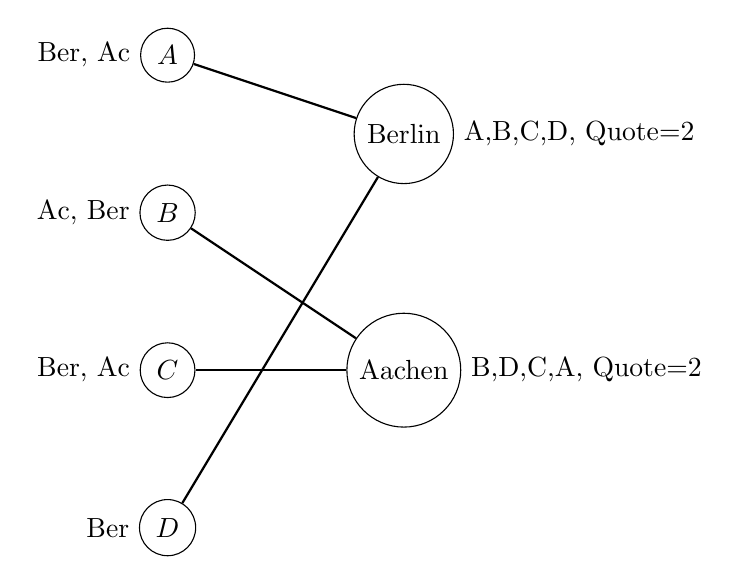
\begin{tikzpicture}
		\node[draw,circle,minimum size=5mm, label = left:{Ber, Ac}] (A) at (0,0) {$A$};
		\node[draw,circle,minimum size=5mm, label = left:{Ac, Ber}] (B) at (0,-2) {$B$};
		\node[draw,circle,minimum size=5mm, label = left:{Ber, Ac}] (C) at (0,-4) {$C$};
		\node[draw,circle,minimum size=5mm, label = left:{Ber}] (D) at (0,-6) {$D$};
		
		\node[draw,circle,minimum size=8mm, label = right:{A,B,C,D, Quote=2}] (Berlin) at (3,-1) {Berlin};
		\node[draw,circle,minimum size=8mm, label = right:{B,D,C,A, Quote=2}] (Aachen) at (3,-4) {Aachen};
	
		\draw[thick] (A) -- (Berlin);
		\draw[thick] (B) -- (Aachen);
		\draw[thick] (C) -- (Aachen);
		\draw[thick] (D) -- (Berlin);
		%\draw[thick,red] (A) -- (Z);
		\end{tikzpicture}
	\end{center}
\end{halfboxr}

\section{Sortieren}

Grundsätzlich in diesem Kapitel, sowie in allen folgenden, beginnen Arrays bzw. Listen immer mit dem Index 0. Das heißt, in einem Array $A$ mit z.B. 3 Elementen, gibt es die Position $A[0]$, $A[1]$ und $A[2]$. Das erste Element eines $n$-elementigen Arrays $A$ ist also $A[0]$ und das letzte $A[n-1]$.

\subsection{Insertion Sort und Merge Sort}

Insertion Sort ist ein Sortierverfahren, dass jedes Element eines Arrays an die richtige Stelle im bereits sortierten Teilarray einfügt (``insertion''). Merge Sort hingegen teilt das Array rekursiv in zwei Teillisten und ``mergt'' diese dann zu sortierten Teillisten zusammen.

\begin{halfboxl}
	\vspace{-\baselineskip}
	\begin{algo}{Insertion Sort}
		\textbf{Eingabe:} Array der Länge $n$
		
		\textbf{Ausgabe:} Aufsteigend sortiertes Array $A$
		\tcblower
		
		\textbf{FOR} $j=1$ \textbf{TO} $n-1$
		
		\tab $key$ = $A[j]$
		
		\tab $i = j-1$
		
		\tab \textbf{WHILE} ($i>0$ \textbf{AND} $A[i]>key$)
		
		\tab\tab $A[i+1] = A[i]$
		
		\tab\tab $i =i-1$
		
		\tab $A[i+1] = key$
		
		\textbf{RETURN} $A$
	\end{algo}
\end{halfboxl}%
\begin{halfboxr}
	\vspace{-\baselineskip}
	\begin{algo}{Merge Sort}
		\textbf{Eingabe:} Array der Länge $n$
		
		\textbf{Ausgabe:} Aufsteigend sortiertes Array $A$
		\tcblower
		
		\textbf{IF} ($n=1$)
		
		\tab \textbf{RETURN} $A$
		
		Sortiere $A[1 \dots \frac{n}{2}]$ und $A[\frac{n}{2} +1 \dots n]$ rekursiv
		
		Merge die beiden sortierten Teilarrays
		
		\textbf{RETURN} $A$
	\end{algo}
\end{halfboxr}

\subsection{Selection Sort und Bubble Sort}

\begin{halfboxl}
	\vspace{-\baselineskip}
	\begin{algo}{Selection Sort}
		\textbf{Eingabe:} Array der Länge $n$
		
		\textbf{Ausgabe:} Aufsteigend sortiertes Array $A$
		\tcblower
		
		\textbf{FOR} $j=0$ \textbf{TO} $n-1$
		
		\tab $i_{\min}$ = $j$
		
		\tab \textbf{FOR} $i = j + 1 $ \textbf{TO} $n-1$
		
		\tab\tab \textbf{IF} ($A[i] < A[i_{\min}]$)
		
		\tab\tab\tab $i_{\min} = i$
		
		\tab \textbf{IF} ($i_{\min} \neq j$)
		
		\tab\tab Tausche $A[j]$ und $A[i_{\min}]$
		
		\textbf{RETURN} $A$
	\end{algo}
\end{halfboxl}%
\begin{halfboxr}
	\vspace{-\baselineskip}
	\begin{algo}{Bubble Sort}
		\textbf{Eingabe:} Array der Länge $n$
		
		\textbf{Ausgabe:} Aufsteigend sortiertes Array $A$
		\tcblower
		
		\textbf{FOR} i = n \textbf{DOWN}\footnotemark \textbf{ TO} 2
		
		\tab \textbf{FOR} j = 0 \textbf{TO} i-1
		
		\tab\tab \textbf{IF} (A[j] $>$ A[j+1])
		
		\tab\tab\tab Tausche A[j] und A[j+1]
		
		\textbf{RETURN} A
	\end{algo}
\end{halfboxr}

\todo[inline]{ Algorithmenboxen schöner machen }

\footnotetext{Das \textbf{DOWN TO} entscheidet sich von den bisherigen \textbf{FOR \dots TO} nur dadurch, dass wir die Variable anstatt hochzuzählen, bei einem \textbf{DOWN TO} nach jeder Iteration der Schleife um eins runterzählen.} 



\section{Laufzeit}

\subsection{Laufzeitanalyse}


Die Laufzeitanalyse untersucht die Dauer, die ein Algorithmus oder Programm zum Lösen eines Problems bzw. einer Eingabe braucht. Da es verschieden schnelle Rechner in verschiedenen Anwendungsgebieten gibt, (z.B. Microcontroller vs Rechencluster), hat man sich darauf geeinigt, die Dauer eines Algorithmus nicht in Sekunden oder Minuten anzugeben, sondern in Abhängigkeit von der Länge der Eingabe. Dabei kommt es auch darauf an, wie ``gut'' die Eingabe codiert ist, aber das würde an dieser Stelle über das Thema hinaus gehen. 

Es gibt drei häufig angewandte Analyse Methoden für Algorithmen:

\begin{itemize}
	\item Worst-Case Analyse: Wie viele Rechenschritte bzw. wie viel Rechendauer benötigt der Algorithmus für die schlimmst-möglichsten Eingabe? Diese Analyseart ist die gängigste und oft auch die aussagekräftigste.
	\item Average-Case Analyse: Wie viele Rechenschritte benötigt der Algorithmus im Durchschnitt für jede Eingabe? 
	\item Best-Case Analyse: Wie viele Rechenschritte benötigt der Algorithmus für die best-mögliche Eingabe? Hier sollte man aufpassen, denn ein "guter" Algorithmus ist nicht nur auf ein paar wenigen Instanzen schnell bzw. effizient.
\end{itemize}

Diese Analysearten sind analog zu den nun folgenden mathematischen Beschreibungen in Form von unteren bzw. oberen Schranken.

\subsection{O-Notation}

Im folgenden wird meist von der Größe oder Länge der Eingabe als $n$ gesprochen. Die Laufzeitanalyse untersucht dann, in welcher Größenordnung sich die Laufzeitfunktion $T(n)$ bei wachsender Eingabegröße $n$ bewegt. Um dies geeignet (aber zugegeben nicht sofort verständlich) darzustellen, wird im Allgemeinen die ``Big-O''-Notation verwendet.



	\begin{defi}{$\mathcal{O}(f)$}
		$\mathcal{O}(f)$ ist die Menge der Funktionen $g$, die nicht schneller wachsen als $f$. Wenn $g\in \mathcal{O}(f)$, ist $c \cdot f(n)$ eine obere Schranke für $g(n)$. Formal aufgeschrieben:
		
		$\mathcal{O}(f):=\{g \in \mathbb{{R}^{\mathbb{N}}_+} | \exists c>0. \exists n_0 \in \mathbb{N}. \forall n \geq n_0 . g(n) \leq c \cdot f(n) \}$
		
		Dabei ist $c$ ein beliebiger Faktor, und $n_0$ ein Wert, ab dem für irgendein $n \geq n_0$ $c \cdot f(n)$ immer größer-gleich $g(n)$ ist. $\mathbb{{R}^{\mathbb{N}}_+}$ liest man als die Menge von Funktionen, die von $\mathbb{N}$ (der Eingabelänge) nach den nicht-negativen reellen Zahlen $\mathbb{R}_+$ (die Laufzeit) auswerten. 
	\end{defi}

	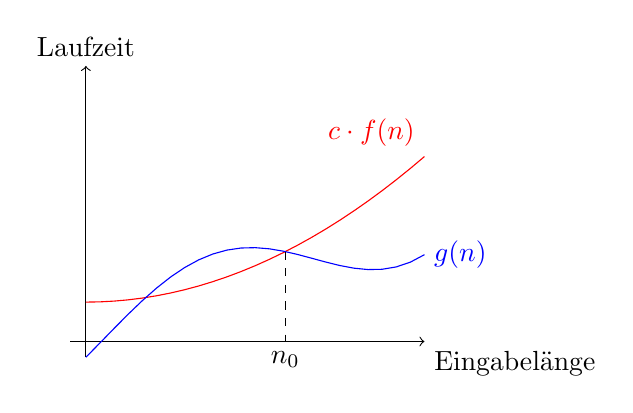
\begin{tikzpicture}[domain=0:4.3] 
	%\draw[thin,color=gray] (-0.1,-1.1) -- (3.9,3.9);
	\draw[->] (-0.2,0) -- (4.3,0) node[below right] {Eingabelänge}; 
	\draw[->] (0,-0.2) -- (0,3.5) node[above] {Laufzeit};
	\draw[color=red]    plot (\x, {0.1*(\x)^2 + 0.5})             node[above left] {$c \cdot f(n)$}; 
	\draw[color=blue]   plot (\x,{sin(\x r)+ 0.12*\x^2 - 0.2})    node[right]{$g(n)$}; 
	
	\draw[dashed] (2.53305, 1.14163) -- (2.53305,0)  node[below] {$n_0$};
	%\draw[color=orange] plot (\x,{0.05*exp(\x)}) node[right] {$f(x) = \frac{1}{20} \mathrm e^x$};
	\end{tikzpicture}
	
	

	\begin{defi}{$\Omega(f)$}
		$\Omega(f)$ ist die Menge der Funktionen $g$, die nicht langsamer wachsen als $f$. Wenn $g\in \Omega(f)$, ist $c \cdot f(n)$ eine untere Schranke für $g(n)$. Formal aufgeschrieben:
		
		$\Omega(f):=\{g \in \mathbb{{R}^{\mathbb{N}}_+} | \exists c>0. \exists n_0 \in \mathbb{N}. \forall n \geq n_0 $ . $g(n) \geq c \cdot f(n) \}$
		
	\end{defi}
	
	\begin{tikzpicture}[domain=0:4.3] 
	%\draw[thin,color=gray] (-0.1,-1.1) -- (3.9,3.9);
	\draw[->] (-0.2,0) -- (4.3,0) node[below right] {Eingabelänge}; 
	\draw[->] (0,-0.2) -- (0,3.5) node[above] {Laufzeit};
	\draw[color=red]    plot (\x, {0.02*(\x)^2 + 0.55})             node[below right] {$c \cdot f(n)$}; 
	\draw[color=blue]   plot (\x,{sin(\x r)+ 0.12*\x^2 + 0.1})    node[above right] {$g(n)$}; 
	
	\draw[dashed] (0.444737, 0.553955) -- (0.444737,0)  node[below] {$n_0$};
	%\draw[color=orange] plot (\x,{0.05*exp(\x)}) node[right] {$f(x) = \frac{1}{20} \mathrm e^x$};
	\end{tikzpicture}


\begin{defi}{$\Theta(f)$}
		$\Theta(f)$ ist die Menge der Funktionen $g$, die nicht langsamer wachsen als $f$. Wenn $g\in \Theta(f)$, ist $c \cdot f(n)$ eine untere Schranke für $g(n)$. Formal aufgeschrieben:
		
		$\Theta(f):=\{g \in \mathbb{{R}^{\mathbb{N}}_+} | \exists c_1,c_2 >0. \exists n_0 \in \mathbb{N}. \forall n \geq n_0 . c_1 \cdot f(n) \leq g(n) \leq c_2 \cdot f(n) \}$
		
		Alternativ gilt: $g \in \Theta(f) \Leftrightarrow g \in \mathcal{O}(f) \land g \in \Omega (f)$
\end{defi}
	
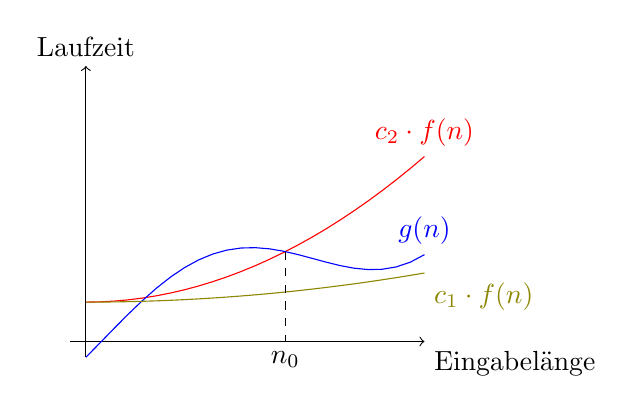
\begin{tikzpicture}[domain=0:4.3] 
	%\draw[thin,color=gray] (-0.1,-1.1) -- (3.9,3.9);
	\draw[->] (-0.2,0) -- (4.3,0) node[below right] {Eingabelänge}; 
	\draw[->] (0,-0.2) -- (0,3.5) node[above] {Laufzeit};
	\draw[color=red]    plot (\x, {0.1*(\x)^2 + 0.5})             node[above] {$c_2 \cdot f(n)$}; 
	\draw[color=blue]   plot (\x,{sin(\x r)+ 0.12*\x^2 - 0.2})    node[above] {$g(n)$}; 
	
	\draw[color=olive]    plot (\x, {0.02*(\x)^2 + 0.50})             node[below right] {$c_1 \cdot f(n)$}; 
	
	\draw[dashed] (2.53305, 1.14163) -- (2.53305,0)  node[below] {$n_0$};
	%\draw[color=orange] plot (\x,{0.05*exp(\x)}) node[right] {$f(x) = \frac{1}{20} \mathrm e^x$};
\end{tikzpicture}

\todo[inline]{Venn-Diagramm mit Beziehungen der einzelnen Mengen}

Laufzeit einiger Algorithmen:

\begin{itemize}
	\item Merge Sort: $\mathcal{O}(n \log (n))$, $\Theta (n \log (n))$
	\item Insertion Sort, Selection Sort: $\mathcal{O}(n^2)$, $\Omega (n)$
\end{itemize}



\section{Interval-Scheduling und Partitioning}

\subsection{Greedy Algorithmen}

Greedy (zu deutsch ``gierig'') Algorithmen ist die Bezeichnung für solche Algorithmen, die versuchen, in jedem Schritt möglichst nah an die optimale Lösung heranzukommen und dabei Stück für Stück eine bessere Lösung generieren. Diese Art der Lösungsfindung funktioniert für einige Probleme gut (z.B. Scheduling, Partitioning), für andere jedoch nicht immer gut (z.B. Cashier's Algorithmus).

\subsection{Cashier's Algorithmus}

Der Cashier's Algorithmus gibt für einen Geldbetrag, das mit Münzen verschiedener Münzwerte ausgezahlt werden soll, eine Menge von Münzen aus, die in Summe gleich dem Geldbetrag sind. 

\begin{algo}{Cashier's Algorithmus}
	\textbf{Eingabe:} Betrag $x$, Münzwerte $c_1, \dots , c_n$
	
	\textbf{Ausgabe:} Menge $S$ an Münzen mit Gesamtwert $x$
	\tcblower
	
	Sortiere die $n$ Münzwerte aufsteigend, sodass $c_1 \leq \dots \leq c_n$
	
	$S = \{ \}$
	
	\textbf{WHILE} ($x>0$)
	
	\tab Sei $k$ der größte Index mit $c_k \leq x$
	
	\tab \textbf{IF} (kein solches $k$ existiert)
	
	\tab\tab \textbf{RETURN} ``keine Lösung''
	
	\tab \textbf{ELSE} 
	
	\tab\tab $x = x - c_k$
		
	\tab\tab Füge eine Münze von Wert $c_k$ zu $S$ hinzu
	
	\tab \textbf{RETURN} $S$
\end{algo}

\begin{theo}{Nicht-Optimalität des Chashier's Algorithmus} Der Cashier's Algorithmus liefert \textit{nicht} immer die optimale Lösung, z.B. würde der Algorithmus nur mit Münzen von Wert 3 und 5 bei einem Betrag von $x=9$ ``keine Lösung'' ausgeben, obwohl drei 3-Münzen möglich sind. 

\end{theo}

\subsection{Interval Scheduling}
Beim Interval Scheduling geht es darum, Anfragen oder Jobs für eine Ressource so auszuwählen, dass sich die Jobs überlappungsfrei sind. Jeder Job $i$ hat dazu eine Startzeit $s_i$ und eine Endzeit $f_i$, oft kurz als $(s_i,f_i)$ angegeben, wobei hier offene Intervalle verwendet werden (d.h., Job (1,3) und Job (3,5) sind überlappungsfrei). Das Ziel ist es dabei, möglichst viele kompatible Jobs auszuwählen. \todo{Insert Defi Block here}

\subsubsection{Interval Scheduling Algorithmus}

Es gibt u.A. die folgenden Auswahlregeln:

\begin{itemize}
	\item[($R1$)] frühester Startzeitpunkt $s_i$
	\item[($R2$)] kürzester Belegungszeitraum $f_i - s_i$
	\item[($R3$)] wenigste Überlappungen mit anderen Intervallen
	\item[($R4$)] frühester Fertigstellungszeitpunkt $f_i$
\end{itemize}

Der grundsätzliche Algorithmus sieht wie folgt aus:

\begin{algo}{Intervall Scheduling}
	\textbf{Eingabe:} Anfragen $M= \{1, \dots , n\}$ für Zeitintervalle $(s_1,f_1), \dots,(s_n,f_n)$
	
	\textbf{Ausgabe:} Kompatible Teilmenge $A$ der Menge $M$
	\tcblower
	
	$A = \{ \}$
	
	\textbf{WHILE} (Die Menge $M$ nicht leer ist)
	
	\tab Wähle eine Anfrage $i$ aus $M$ gemäß einer Auswahlregel $(R_*)$
	
	\tab Füge $i$ zu $A$ hinzu
	
	\tab Lösche alle mit $i$ überlappenden Intervalle aus $M$, inklusive $i$
	
	\textbf{RETURN} $A$
\end{algo}

Es wird hier davon ausgegangen, dass innerhalb des Algorithmus nicht mehrere, sondern immer nur eine Auswahlregel angewandt wird.

\subsubsection{Optimaler Inverall Scheduling Algorithmus}

Der Earliest-Finish-Time-First Algorithmus, der der Auswahlregel $(R4)$ von oben entspricht, liefert stets eine optimale Lösung. Die folgende Implementierung hat dabei die Laufzeit von $\mathcal{O}(n \cdot \log (n))$:

\begin{algo}{Earliest-Finish-Time-First}
	\textbf{Eingabe:} Anfragen $M= \{1, \dots , n\}$ für Zeitintervalle $(s_1,f_1), \dots,(s_n,f_n)$
	
	\textbf{Ausgabe:} Kompatible Teilmenge $A$ der Menge $M$
	\tcblower
	
	Sortiere und re-indiziere die Intervalle, sodass $f_1 \leq \dots \leq f_n$
	
	$A = \{ \}$
	
	\textbf{FOR} ( $j = 1$ \textbf{TO} $n$)
	
	\tab \textbf{IF} ($j$ ist kompatible mit $A$)
	
	\textbf{RETURN} $A$
\end{algo}

An dieser Stelle nicht davon verwirren lassen, dass wir zwei verschiedene Implementierungen für den gleichen Algorithmus verwenden. Oft gibt es mehrere Algorithmen, die das gleiche Konzept umsetzen. Hier unterscheiden sich die beiden Varianten dadurch, dass bei der zweiten die Intervalle vorher noch sortiert werden, was bei der ersten nicht gemacht wird. 

 
\subsection{Intervall Partitioning}

Das Intervall Partitioning Problem ist ähnlich zu dem Intervall Scheduling Problem, jedoch ist es hier das Ziel, \textit{alle} Jobs so auf mehrere (nicht nur eine) Ressource aufzuteilen, dass alle Jobs auf einer Ressource kompatibel sind und wir möglichst wenig Ressourcen verwenden. \todo{insert defi block here}

\subsubsection{Intervall Partitioning Algorithmus}

Analog zum Scheduling gibt es hier auch folgende Auswahlregeln:

\begin{itemize}
	\item[($R1$)] frühester Startzeitpunkt $s_i$
	\item[($R2$)] kürzester Belegungszeitraum $f_i - s_i$
	\item[($R3$)] wenigste Überlappungen mit anderen Intervallen
	\item[($R4$)] frühester Fertigstellungszeitpunkt $f_i$
\end{itemize}

Der grundsätzliche Algorithmus sieht dabei wie folgt aus:

\begin{algo}{Intervall Partitioning}
	\textbf{Eingabe:} Anfragen $M= \{1, \dots , n\}$ für Zeitintervalle $(s_1,f_1), \dots,(s_n,f_n)$
	
	\textbf{Ausgabe:} Schedule $S$ bei dem alle paarweise überlappenden Intervalle unterschiedlichen Ressourcen zugewiesen wurden
	\tcblower
	
	Sortiere und re-indiziere die Anfragen in $M$ gemäß der ausgewählten Prioritätsregel $(R_*)$. Nummeriere die Anfragen dann mit $1,\dots, n$ durch.
	
	Setze $d=0$
	
	\textbf{FOR} ($i = 1$ \textbf{TO} $n$)
	
	\tab \textbf{IF} ($i$ kann einer der Ressourcen $d$ kompatibel zugewiesen werden)
	
	\tab\tab Weise $i$ einer solchen Ressource zu
	
	\tab \textbf{ELSE}
	
	\tab\tab Stelle eine weitere Ressource $d+1$ zur Verfügung
	
	\tab\tab Weise $i$ dieser neuen Ressource $d+1$ zu
	
	\tab\tab $d= d+1$

	
	\textbf{RETURN} den resultierenden Schedule $S$
\end{algo}

\begin{theo}{Optimaler Intervall Partitioning Schedule}
	Die Auswahlregel $(R1)$- frühester Startzeitpunkt - liefert stets einen optimalen Schedule. Sie wird auch \emph{Earliest-Start-Time-First} gennant. Bei den anderen Auswahlregeln wird \emph{nicht} immer ein optimale Schedule bestimmt. 
\end{theo}

\begin{halfboxl}
	\vspace{-\baselineskip}
	\begin{defi}{Tiefe einer Instanz}
		Die \emph{Tiefe} einer Instanz $M$ (kurz: Tiefe($M$)) ist die maximale Kardinalität einer Teilmenge $A$ der Anfragen aus $M$, sodass es einen Zeitpunkt $t$ gibt, der in allen Intervallen aus $A$ enthalten ist. 
		
		Also gibt die Tiefe die Anzahl der Ressourcen, die wir \emph{mindestens} für einen Schedule benötigen. 
	\end{defi}
\end{halfboxl}%
\begin{halfboxr}
	\vspace{0.2cm}
	\begin{tightcenter}
		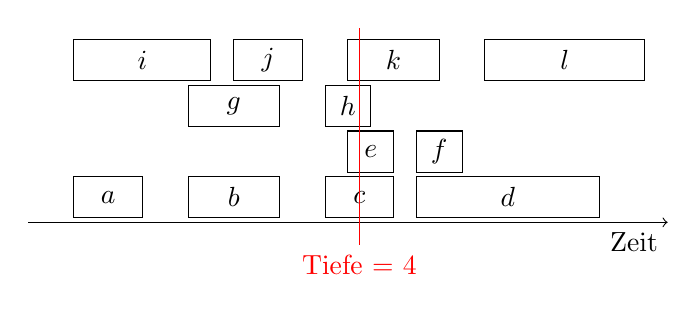
\begin{tikzpicture}[scale=.58]%[x=1.7cm,y=1cm]
		\draw[->] (-.5,1) -- (13.5,1) node[below left] {Zeit};
		
		\draw (.5,1.1) rectangle (2,2) node[midway] {$a$};
		\draw (3,1.1) rectangle (5,2) node[midway] {$b$};
		\draw (6,1.1) rectangle (7.5,2) node[midway] {$c$};
		\draw (8,1.1) rectangle (12,2) node[midway] {$d$};
		
		\draw (6.5,2.1) rectangle (7.5,3) node[midway] {$e$};
		\draw (8,2.1) rectangle (9,3) node[midway] {$f$};

		
		\draw (3,3.1) rectangle (5,4) node[midway] {$g$};
		\draw (6,3.1) rectangle (7,4) node[midway] {$h$};
		
		\draw (.5,4.1) rectangle (3.5,5) node[midway] {$i$};
		\draw (4,4.1) rectangle (5.5,5) node[midway] {$j$};
		\draw (6.5,4.1) rectangle (8.5,5) node[midway] {$k$};
		\draw (9.5,4.1) rectangle (13,5) node[midway] {$l$};

		\draw[color=red] (6.75, 5.25) -- (6.75,0.5)  node[below] {Tiefe = 4};
		
		\end{tikzpicture}
	\end{tightcenter}
\end{halfboxr}

\subsection{Scheduling zur Minimierung von Verspätung}

Als letztes Thema in diesem Kapitel betrachten wir folgendes Problem: Es gibt wie vorher auch $n$ Jobs, die aber wieder nur auf einer Ressource abgearbeitet werden sollen. Es können die Jobs nur nacheinander abgearbeitet werden, nicht gleichzeitig und alle Jobs können jederzeit begonnen werden, haben also keinen Startzeitpunkt wie zuvor. Jeder Job $j$ hat eine Bearbeitungszeit $p_j$ und eine Deadline $d_j$, zu der er möglichst fertig sein soll. Wenn ein Job $j$ also zum Zeitpunkt $s_j$ beginnt, ist er zum Zeitpunkt $f_j = s_j + p_j$, also Startzeit plus Bearbeitungszeit, fertig. Falls der Job nach seiner Deadline abgeschlossen wurde, hat er eine Verspätung von $f_j - d_j$, also Fertig-Zeitpunkt minus Deadline. Ist der Job vor seiner Deadline fertig geworden, weisen wir ihm die Verspätung 0 zu. Kurz gefasst hat jeder Job also die Verspätung $l_j = \max \{0, f_j - d_j\}$.  \todo{Das ganze in eine Definition packen}

Das Ziel ist es nun, einen Schedule zu finden, sodass die maximale Verspätung, die irgendein Job $j$ hat, zu minimieren (nicht die Summe der Verspätungen aller Jobs!). Mathematisch: Minimiere $L = \max_{j \in J} \{l_j\}$. Es ist hier also \emph{besser}, wenn alle Jobs eine Verspätung von 2 Zeiteinheiten hätten, als wenn ein Job eine Verspätung von 4 Einheiten hat, aber alle anderen vor ihrer Deadline fertig geworden sind. 

Wir haben erneut Auswahlregeln, aber da wir nun keine festen Startzeitpunke haben, fällt ``Earliest-Start-Time-First'' weg:

\begin{itemize}
	\item Shortest-Processing-Time-First: Schedule die Aufträge aufsteigend in der Reihenfolge ihrer Bearbeitungszeiten $p_j$, angefangen beim kürzesten
	\item Earliest-Deadline-First: Schedule die Aufträge aufsteigend in der Reihenfolge ihrer Deadlines $d_j$
	\item Smallest-Slack: Schedule die Aufträge austeigend in der Reihenfolge ihres ``Slack'' $d_j - p_j$
\end{itemize} 

\begin{theo}{Optimalität von Earliest-Deadline-First}
	Für die minimierung von Verspätung ist Earliest-Deadline-First die optimale Auswahlregel, die anderen beiden generieren nicht immer optimale Schedules
\end{theo}

\begin{algo}{Earliest-Deadline-First (Minimierung von Verspätungen)}
	\textbf{Eingabe:} Aufträge $M= \{1, \dots , n\}$ mit Processing Time $p_j$ und Deadline $d_j$
	
	\textbf{Ausgabe:} Schedule $S$ 
	
	\tcblower
	
	Sortiere und re-indiziere die $n$ Aufträge in aufsteigender Reihenfolge der Deadlines $d_j$
	
	Setze $t=0$
	
	\textbf{FOR} ($i = 1$ \textbf{TO} $n$)
	
	\tab Schedule Auftrag $j$ im Intervall $[t, t+ p_j]$
	
	\tab $s_j = t$ \textit{ \color{gray} // speichere Start- und }
	
	\tab $f_j = s_j + p_j$  \textit{ \color{gray} // Endzeitpunkt ab }
	
	\tab $t = t + p_j$  \textit{ \color{gray} // setze $t$ auf den nächsten freien Zeitpunkt }
	
	
	\textbf{RETURN} den resultierenden Schedule $S$
\end{algo}

\section{Graphentheorie}

\subsection{Der langweilige Teil - Definitionen}

\subsubsection{Grundlegende Notation}

Es folgen ein paar langweilige Definitionen.

\begin{halfboxl}
	\vspace{-\baselineskip}
	\begin{defi}{Gerichteter Graph}
		Ein gerichteter Graph (auch: Digraph) $G$ ist ein Paar $(V,A)$ mit:
		
		\begin{itemize}
			\item Einer endlichen Menge $V$ von Knoten (``Vertices'')
			
			\item Einer Menge $A$ von \emph{geordneten} Paaren (Tupel) von Knoten, die (gerichtete) Kanten oder Bögen (``arcs'') genannt werden.
		\end{itemize}
	
	Man verwendet gerichtete Graphen zur Darstellung asymmetrischer Beziehungen zwischen zwei Knoten, z.B. Einbahnstraßen 
	\end{defi}
\end{halfboxl}%
\begin{halfboxr}
	\vspace{-\baselineskip}
	\begin{defi}{Ungerichteter Graphen}
		Ein ungerichteter Graph $G$ ist ein Paar $(V,E)$ mit:
		
		\begin{itemize}
			\item Einer endlichen Menge $V$ von Knoten (``Vertices'')
			
			\item Einer Menge $A$ von \emph{ungeordneten} Paaren von Knoten, die (gerichtete) Kanten (``edges'') genannt werden.
		\end{itemize}
	
	Man verwendet ungerichtete Graphen zur Darstellung symmetrischer Beziehungen zwischen zwei Knoten, z.B. Freundschaften
	\end{defi}
\end{halfboxr}

\begin{thirdboxl}
	\vspace{-\baselineskip}	
	\begin{defi}{Adjazent/benachbart}
	Sind $u$ und $v$ die beiden Endknoten einer [gerichteten] Kante $e = \{u,v\}$ [$a= (u,v)$], so ist $v$ \emph{adjazent} oder \emph{``benachbart''} zu $u$.
	
	Die Knoten $u$ und $v$ sind dann \emph{inzident} zur [gerichteten] Kante $e = \{u,v\}$ [$a= (u,v)$].
	\end{defi}

	\begin{defi}{Vollständig/Symmetrisch}
		Ein Graph $G$ heißt \emph{vollständig}, wenn jedes Knotenpaar durch eine Kante verbunden ist.
		
		Ein gerichteter Graph heißt \emph{symmetrisch}, wenn für jede Kante $(u,v) \in A$ auch die ``Rückweg-Kante'' $(v,u) \in A$.
	\end{defi}
\end{thirdboxl}%
\begin{thirdboxm}
	\vspace{-\baselineskip}		
	\begin{defi}{Grad eines Knoten}
		Der \emph{Grad} $\deg (u)$ eines Knoten ist die Anzahl der Kanten, die an ihn angrenzen. Schlaufen werden doppelt gezählt
		
		Bei gerichteten Graphen unterscheidet man zwischen der Anzahl der eingehenden Kanten $\deg ^- (u)$ und der ausgehenden Kanten $\deg ^+ (u)$.
	\end{defi}

	\begin{theo}{Handshaking Lemma}
		In einem ungerichteten Graphen $G = (V,E)$ gilt:
		
		$\sum_{v \in V} \deg (v) = 2 \cdot |E|$
	\end{theo}
\end{thirdboxm}%
\begin{thirdboxr}
	\vspace{-\baselineskip}	
	\begin{defi}{induzierter Teilgraph}
		Ein Teilgraph eines Graphe $G = (V,E)$ ist ein Graph $G' = (V',E')$ mit $V'$ ist eine Teilmenge von $V$ und $E'$ ist eine Teilmenge von $E$. 
		
		Der Teilgraph $G' = (V',E')$ heißt induzierter Teilgraph, wenn $E'$ alle Kanten aus $E$ enthält, deren beide Endpunkte in $V'$ sind.
	\end{defi}
	
	\begin{defi}{Schlaufe}
		Eine Kante mit zwei Identischen Endknoten wird \emph{Schlaufe} oder \emph{Schlinge} genannt.
	\end{defi}
	
\end{thirdboxr}

\subsubsection{Wege, Kreise, Bäume}

Es folgen weitere, noch mehr langweilige Definitionen

\begin{thirdboxl}
	\vspace{-\baselineskip}	
	\begin{defi}{Weg/Pfad}
		Ein \emph{Weg} (oder \emph{Pfad}) in einem [gerichteten] Graphen $G = (V,E)$ [$G = (V,A)$] von einem Knoten $v$ zu einem Knoten $w$ ist eine Sequenz an Knoten $v, x_1, x_2, \dots , x_n, w$, wobei je zwei aufeinanderfolgende Knoten durch eine [gerichtete] Kante verbunden sind.
	\end{defi}
	
	\begin{defi}{Einfache Wege}
		Ein Weg ist \emph{einfach}, wenn alle Knoten auf dem Weg paarweise unterschiedlich sind.
	\end{defi}
\end{thirdboxl}%
\begin{thirdboxm}
	\vspace{-\baselineskip}		
	\begin{defi}{Zusammenhang (ungerichtete Graphen)}
		Ein Knoten $w$ ist vom Knoten $v$ aus \emph{erreichbar}, wenn es einen Weg von $v$ nach $w$ gibt.
		
		Ein ungerichteter Graph $G= (V,E)$ ist \emph{zusammenhängend}, wenn jeder Knoten von jedem anderen Knoten aus erreichbar ist.
		
		Eine \emph{Zusammenhangskomponente} eines ungerichteten Graphen $G$ ist ein maximal zusammenhängender Teilgraph.
	\end{defi}
	
\end{thirdboxm}%
\begin{thirdboxr}
	\vspace{-\baselineskip}	
	\begin{defi}{Zusammenhang (gerichtete Graphen)}
		Ein Knoten $w$ ist vom Knoten $v$ aus \emph{erreichbar}, wenn es einen Weg von $v$ nach $w$ gibt.
		
		Ein gerichteter Graph $G= (V,A)$ ist \emph{stark zusammenhängend}, wenn jeder Knoten von jedem anderen Knoten aus erreichbar ist.
		
		Eine \emph{starke Zusammenhangskomponente} eines gerichteten Graphen $G$ ist ein maximal stark zusammenhängender Teilgraph.
	\end{defi}
	
\end{thirdboxr}

\todo[inline]{Beispiele dazu?}

\begin{halfboxl}
	\vspace{-\baselineskip}
	\begin{defi}{Kreise}
		Ein \emph{Kreis} in einem ungerichteten Graph $G=(V,E)$ ist ein Weg mit gleichem Start- und Endknoten
		
		Ein Kreis ist \emph{einfach}, wenn die Zwischenknoten paarweise verschieden sind.
	\end{defi}

	\begin{theo}{Relation von Bäumen und Wäldern}
		Ein Baum-Graph ist auch stets ein Wald, aber ein Wald-Graph ist nicht immer auch ein Baum, da ein Wald aus mehreren Bäumen bestehen kann.
	\end{theo}

	
\end{halfboxl}%
\begin{halfboxr}
	\vspace{-\baselineskip}
	\begin{defi}{Bäume und Wälder}
		Ein ungerichteter (Teil-)Graph $G= (V,E)$ wird \emph{Baum} genannt, wenn $G$ kreisfrei und zusammenhängend ist.
		
		Ein kreisfreier ungerichteter Graph $G=(V,E)$ wird \emph{Wald} genannt.
	\end{defi}

	\begin{theo}{Knotenzahl eines Baumes}
		Ein Baum mit $n$ Knoten hat $n-1$ Kanten
	\end{theo}

	
\end{halfboxr}

\subsubsection{Darstellung von Graphen}

Es gibt mehrere Möglichkeiten, Graphen zu kodieren, das heißt einfach verständlich für Menschen bzw. Computer aufzuschreiben:

	\begin{defi}{Adjazenmatrix}
		Graphen können mittels \emph{Adjazenzmatrizen} repräsentiert und gespeichert werden:
		
		\begin{itemize}
			\item Die Adjazenzmatrix zum Graphen $G = (V,E)$ [$G=(V,A)$] mit Knotenmenge $V= \{1,\dots, n\}$ ist eine Matrix, deren Einträge entweder 0 oder 1 sind, und die $n$ Zeilen und $n$ Spalten hat, wobei
			
			\item der Eintrag in Zeile $i$, Spalte $j$ genau dann $1$ ist, wenn die beiden Knoten $i$ und $j$ durch eine ungerichtete Kante verbunden sind bzw. eine gerichtete Kante von $i$ nach $j$ verläuft.
		\end{itemize}
	
	Adjazenzmatrizen eignen sich gut für die Verarbeitung in Programmen.
	\end{defi}

\begin{halfboxl}
	\vspace{-\baselineskip}		
	\begin{defi}{Explizite Angabe}
		Die explizite Angabe meint, dass man einen Graphen $G= (V,E)$ durch explizites Aufschreiben der Mengen $V$ und $E$ [bzw. $A$] angibt.
		
		Beispiel: 
	\end{defi}
	
\end{halfboxl}%
\begin{halfboxr}
	\vspace{-\baselineskip}	
	\begin{defi}{Skizze}
		Die Angabe durch Skizze meint, den Graphen aufzuzeichnen. Diese Art eignet sich sehr gut für Menschen.
		
		Beispiel: 
	\end{defi}
	
\end{halfboxr}
\todo[inline]{Beispiel} 

Es gibt außerdem noch die Möglichkeit, statt Adjazenmatrizen auch Adjazenzlisten zu verwenden, die etwas effizienter im Speicherverbrauch sind (folgt eventuell noch an dieser Stelle).

\subsection{Der spaßige Teil - Algorithmen}

\subsubsection{Breitensuche}

Breitensuche ist für viele (``kleine'') Graphenprobleme die Allzweckwaffe schlechthin. Anwendungen sind zum Beispiel die Bestimmung von Zusammenhangskomponenten, Topologische Sortierung, Kritische-Pfad-Analyse, kürzeste-Wege Suche (\emph{nur} wenn alle Kanten Gewicht 1 haben) oder die Verifikation von Regular Safety Properties für endliche Transitionssysteme (\textit{letzteres ist nicht Teil dieser Veranstaltung}). Die Idee ist, ausgehend von einem Startknoten $s$, nacheinander alle Knoten Schicht für Schicht hinzuzufügen.

\begin{algo}{Breitensuche (BFS)}
	\textbf{Eingabe:} Ein Graph $G$ sowie einen Startknoten $s$
	
	\textbf{Ausgabe:} Knoten in den einzelnen Schichten ausgehen von Startknoten $s$
	
	\tcblower
	
	Markiere alle Knoten als ``unbesucht''
	
	Markiere Startknoten $s$ als ``besucht'' und setze $L_0 = \{s\}$
	
	$i=0$
	
	\textbf{WHILE} (es noch unbesuchte Narchbarn von Knoten in $L_i$ gibt)
	
	\tab $L_{i+1} = \{\texttt{alle unbesuchten Nachbarn von } L_i \}$
	
	\tab Markiere die Knoten in $L_{i+1}$ als ``besucht''
	
	\tab $i = i+1$
	
	\textbf{RETURN} $L_k$ $\forall k \in \{0, \dots, i\}$
\end{algo}

\subsubsection{Dijkstra}

Der Dijkstra-Algorithmus steht der Breitensuche im Coolness-Faktor um nichts nach, und wird vor allem zum Lösen des kürzeste-Wege Problem benutzt:

\begin{defi}{Kürzeste-Wege Problem}
	\begin{itemize}
		\item Gerichteter Graph $G= (V,A)$
		\item Kantenlänge $c(a)\geq 0$ auf allen Kanten $a \in A$
		\item Ein Startknoten $s \in V$ und einen Zielknoten $t \in V$
	\end{itemize}

	Gesucht ist ein kürzester Weg von $s$ zu $t$.
\end{defi}

\begin{halfboxl}
	\boxspace
Damit Dijkstra jedoch seine ganze Coolness entfalten kann, müssen ein paar Bedingungen für einen Graphen $G$ gelten:

\begin{theo}{Voraussetzungen für Dijkstra}
\begin{itemize}
	\item Alle Knoten in $G = (V,A)$ sind von $s$ aus erreichbar
	\item Es gibt weder Schleifen, noch parallele Kanten
	\item Es gibt keine negativen Kantengewichte $c(a)$ für $a \in A$
\end{itemize}

Die ersten beiden Voraussetzungen sind durch Preprocessing immer möglich herzustellen.

\end{theo}

\end{halfboxl}%
\begin{halfboxr}
	\boxspace
Der Algorithmus verwendet außerdem eine eigene Notation (weil er cool ist):

	\vspace{\baselineskip}
\begin{defi}{Notation für Dijkstra}
	\begin{itemize}
		\item $S$: Alle Knoten $u \in V$, für die bereits ein kürzester $s-u$-Weg berechnet wurde
		\item $d(u)$: Länge eines kürzesten $s-u$-Weges (Distanz)
		\item $N(S)$: Nachbarn von $S$, d.h. diejenigen Knoten, die von einem Knoten $S$ aus über eine Kante erreichbar sind
	\end{itemize}
\end{defi}
\end{halfboxr}

Wir kommen zum eigentlichen Algorithmus (der auch die kürzesten Wege ausgibt):

\begin{algo}{Dijkstra-Algorithmus }
	\textbf{Eingabe:} Ein gerichteter Graph $G = (V,A)$ mit zugeh. Kantenkosten $c(a)$ und einen Startknoten $s$
	
	\textbf{Ausgabe:} Den kürzesten Weg $p(v)$ vom Startknoten $s$ zum Knoten $v$ und seine Länge $d(v)$ für jeden Knoten $v \in V$
	
	\tcblower
	
	Initialisiere $S = \{s\}$ und $d(s) = 0$
	
	\textbf{WHILE} ($S \neq V$)
	
	\tab \textbf{FOR} (jeden Nachbarn $n \in N(S)$)
	
	\tab\tab Berechne vorläufige Distanz $d'(n) = \min \{d(u) + c(u,n) | u \in S, (u,n) \in A \}$
	
	\tab Wähle Knoten $n$ mit minimaler vorläufiger Distanz $d'(n)$
	
	\tab Füge $n$ zu $S$ hinzu
	
	\tab Setze $d(n) = d'(n)$ und $p(n) = u$ \textit{ \color{gray} // Speichere den Vorgänger von $n$ in $p(n)$ ab }
	
	\textbf{RETURN} $d(v), p(v)$ $\forall v \in V$
\end{algo}

Es bietet sich an, die Zwischenschritte von Dijkstra in einer geeigneten Tabelle festzuhalten.

\begin{theo}{Korrektheit von Dijkstra}
	Zu jeder Zeit während des Algorithmus gilt, für einen Knoten $u \in S$, dass der Wert $d(u)$ der Länge eines kürzesten $s-u$-Weges entspricht.	
\end{theo}

\section{Minimale Spannbäume}

\subsection{Problemdefinition}

\begin{defi}{Das Minimal-Spanning-Tree (MST) Problem}
	Gegeben ist ein ungerichteter zusammenhängender Graph $G= (V,E)$ mit nicht-negativen Kantenkosten $c_e$ für alle $e \in E$
	
	Gesucht ist eine Kanten-Teilmenge $T \subseteq E$ mit minimalen Kosten $\sum_{e \in T} c_e$, sodass der Teilgraph $G[T] = (V,T)$ zusammenhängend ist. 
	
	Dabei gibt es stets eine optimale Lösung $T \subseteq E$, wodurch $G[T] = (V,E)$ ein Baum ist. Deswegen spricht man von Minimalen Spann\emph{bäumen}.
\end{defi}

\subsection{Hilfreiche Eigenschaften von Bäumen und der Austauschsatz}

\begin{theo}{Eigenschaften eines Baumes}
	Die folgenden vier Aussagen sind für einen ungerichteten Graphen $G= (V,E)$ äquivalent (d.h. jede Aussage impliziert alle anderen):

	\begin{enumerate}
		\item $G=(V,E)$ ist ein Baum
		\item Je zwei Knoten in $V$ sind durch genau einen weg verbunden
		\item $|T| = |V| - 1$ und der Graph $G = (V,E)$ ist zusammenhängend
		\item $|T| = |V| - 1$ und der Graph $G = (V,E)$ ist kreisfrei
	\end{enumerate}
\end{theo}

\begin{halfboxl}
	\boxspace
	
	\begin{defi}{Abkürzende Schreibweise}
		Sei $F$ eine Teilmenge von $E$. Weiter seien $e \in F$ und $f \in E\setminus F$. Wir bezeichnen mit:
		
		\begin{itemize}
			\item $F + e$ die Menge, die aus $F$ ensteht, wenn man $e$ hinzufügt,
			\item $F -f$ die Menge, die aus $F$ entsteht, wenn man $f$ entfernt
		\end{itemize}
		
	\end{defi}
	
\end{halfboxl}%
\begin{halfboxr}
	\boxspace
	
	\begin{defi}{Austauschlemma}
		Sei $(V,T)$ ein aufspannender Baum im ungerichteten Graphen $G = (V,E)$. Sei $e \in E$ eine Kante, die nicht in $T$ liegt. Dann gilt:
		
		\begin{itemize}
			\item Der Teilgraph $(V,T+e)$ enthält genau einen Kreis $C$
			\item Für jede Kante $f$ aus dem Kreis $C$ gilt, das $(V,T+e-f)$ ein aufspannender Baum ist.
		\end{itemize}
	\end{defi}
	
\end{halfboxr}

\todo[inline]{Eventuell Graph wie in Vorlesung für das Austauschlemma?}

\subsection{Algorithmen zum Finden eines MSTs}

Zum finden eines MSTs betrachten wir im folgenden zwei Algorithmen, Kruskal und Prim. Kruskal wählt streng nach dem greedy-Prinzip die Kanten in der aufsteigenden Reihenfolge ihrer Kosten und prüft dabei, ob eine neue Kante ein Kreis verursachen würde. Prim hingegen baut den MST anhand von bereits gewählten Kanten mit Hilfe des Schnittes auf.

\subsubsection{Kruskal}

\begin{algo}{Kruskal}
	\textbf{Eingabe:} Ein ungerichteter zusammenhängender Graph $G = (V,E)$ mit nicht-negativen Kantenkosten $c(e)$ $\forall e \in E$
	
	\textbf{Ausgabe:} Eine kostengünstigste Teilmenge $T$ der Kanten, sodass der Teilgraph $G[T] = (V,E)$ zusammen-hängend ist
	
	\tcblower
	
	$T = \{ \}$ \textit{ \color{gray} // $T$ enthält diejenigen Kanten, die der Algorithmus wählt }
	
	$E' = E$ \textit{ \color{gray} // $E'$ enthält die Kanten, die noch nicht betrachtet wurden }
	
	\textbf{WHILE} ($|T| < |V| - 1$)
	
	\tab Wähle günstigste Kante $e \in E'$
	
	\tab Entferne $e$ aus $E'$
	
	\tab \textbf{IF} ($T+e$ kreisfrei)
	
	\tab\tab Füge $e$ zu $T$ hinzu
		
	\textbf{RETURN} $T$
\end{algo}

\subsubsection{Prim}

Für den Algorithmus von Prim benötigen wir vorher noch die Definition des Schnitts einer Knotenmenge

\begin{halfboxl}
	\boxspace
\begin{defi}{Schnitt}
	Sei $G=(V,E)$ ein ungerichteter Graph und $S$ eine Teilmenge der Knoten. Die Menge aller Kanten aus $E$, die genau einen Endknoten in $S$ besitzen, wird auch \emph{Schnitt von $S$} oder \emph{Schnitt($S$)} genannt.
\end{defi}

\end{halfboxl}%
\begin{halfboxr}
	\boxspace
	
	\begin{theo}{Schnitte und Kreise}
		Schnitte und Kreise haben stets eine gerade Anzahl an gemeinsamen Kanten
	\end{theo}
\end{halfboxr}

\todo[inline]{Beispiel für Schnitt}

\begin{algo}{Prim}
	\textbf{Eingabe:} Ein ungerichteter zusammenhängender Graph $G = (V,E)$ mit nicht-negativen Kantenkosten $c(e)$ $\forall e \in E$
	
	\textbf{Ausgabe:} Eine kostengünstigste Teilmenge $T$ der Kanten, sodass der Teilgraph $G[T] = (V,E)$ zusammen-hängend ist
	
	\tcblower
	
	$T = \{ \}$ \textit{ \color{gray} // $T$ enthält diejenigen Kanten, die der Algorithmus wählt }
	
	Wähle einen beliebigen Startknoten $s$ und setze $S = \{s\}$
	
	\textbf{WHILE} ($|T| < |V| - 1$)
	
	\tab Wähle günstigste Kante $e$ aus dem Schnitt von $S$

	\tab Füge $e$ zu $T$ hinzu
	
	\tab Erweitere $S$ um den fehlenden Endknoten von $e$
	
	\textbf{RETURN} $T$
\end{algo}

\subsubsection{Key-Lemma}

Der folgende Abschnitt behandelt das Key-Lemma, welches für den Beweis der Korrektheit von Kruskal und Prim verwendet wird. Die diese Beweise jedoch über den Umfang dieses Horizont hinaus gehen, soll das Key-Lemma hier nur kurz erwähnt werden.

\begin{defi}{Key-Lemma}
	Eine Teilmenge $F$ der Kantenmenge $E$ ist \emph{MST-geeignet}, wenn es einen MST gibt, der alle Kanten aus $F$ enthält. 
	
	Sei $F$ eine MST-geeignete Kantenmenge bzgl. eine Graphen $G = (V,E)$ mit Kantenkosten $c$. dann gilt für jede Knotenmenge $U$, die eine Zusammenhangskomponente des Graphen $(V,F)$ induziert:
	
	Ist $e$ eine günstige Kante im Schnitt von $U$, dann ist $F+e$ MST-geeignet.
\end{defi}

\todo[inline]{Beispiel Key-lemma}

\begin{theo}{Korrektheit Kruskal und Prim}
	Kruskal und Prim liefen garantiert immer einen MST.
\end{theo}

\subsection{Clustering}

\subsubsection{Das Clustering Problem}

\begin{defi}{Das Clustering Problem}
	Ziel: Gruppiere eine Menge an (vergleichbaren) Objekten, z.B. Websiten oder Bilder.
	
	Annahmen:
	\begin{itemize}
		\item Es gibt für zwei Objekte $u$ und $v$ einen Distanzwert $d(u,v)$, der die Ähnlichkeit bzw. Unterschiedlichkeit zwischen $u$ und $v$ beschreibt
		\item Das Distanzmaß ist symmetrisch, d.h. $d(u,v) = d(v,u)$ für alle Objektpaare $\{u,v\}$
		\item Die Objekte sollen in $k$ Cluster eingeteilt werden
	\end{itemize}
\end{defi}

Um ein Merkmal der ``Qualität'' einer Aufteilung von Objekten in $k$ Cluster (``Clustering'') zu haben, betrachten wir hier zunächst das \emph{Max-k-Spacing-Clustering} Problem, um dann die Qualität eines Clustering zu definieren:

\begin{defi}{Max-k-Spacing-Clustering}
	Gegeben ist eine Menge $U = 1,\dots, n$ an Objekten, eine natürliche Zahl $k$ und die Distanzen $d(u,v)$ für alle Objekte $u,v$ aus $U$
	
	Gesucht ist ein Clustering der Objekte in $U$ in $k$ nicht-leere Cluster, sodass die minimale Distanz zwischen zwei Objekten aus unterschiedlichen Clustern möglichst groß ist. 
	
	Das Ziel ist es also, die Cluster so festzulegen, dass die (kürzeste) Distanz zwischen zwei Cluster möglichst groß ist
\end{defi}

\begin{defi}{Spacing}
	Sei $\mathcal{C} = C_1 \cup \dots \cup C_k$ ein Clustering der Objekte aus $U$ in $k$ paarweise disjunkte Cluster. $C$ wird dann auch ein $k$-Clustering der Menge $U$ genannt.
	
	Als \emph{spacing} (oder ``Qualität'') eines Clustering $\mathcal{C} = C_1 \cup \dots \cup C_k$ wird die minimale Distanz zweier Obkekte aus unterschiedlichen Clustern bezeichnet, d.h.,
	
	\centering spacing $(\mathcal{C}) = \min \{d(u,v) | u \in C_i, v \in C_j,$ für $i \neq j \}$
\end{defi}

\todo[inline]{Beispiel für Clustering}

\subsubsection{Max-k-Spacing-Clustering Algorithmus}

\begin{algo}{Max-k-Spacing-Clustering Algorithmus}
	\textbf{Eingabe:} Menge $U$ an $n$ Objekten, natürliche Zahl $k$, Distanz $d(u,v)$ zwischen allen Knoten $u,v \in U$
	
	\textbf{Ausgabe:} Eine Aufteilung der Objekte in $U$ in $k$ nicht-leere Cluster
	
	\tcblower
	
	Konstruiere einen Graphen mit $n$ Knoten, die die Objekte in $U$ repräsentieren und ohne Kanten.
	
	\textit{ \color{gray} // Der initiale Graph besteht somit aus $n$ Zusammenhangskomponenten }
	
	\textbf{WHILE} (es mehr als $k$ Zusammenhangskomponenten (Cluster) gibt)
	
	\tab Wähle zwei Knoten aus unterschiedlichen Clustern, deren Distanz minimal ist
	
	\tab Verbinde diese Knoten durch eine Kante
	
	\tab \textit{ \color{gray} // Somit gibt es ein Cluster weniger }
	
	\textbf{RETURN} die $k$ Cluster $C_1, \dots, C_k$
\end{algo}

\begin{halfboxl}
	\boxspace
	
	\begin{theo}{Äquivalenz des Algorithmus zu Kruskal}
		Der max-k-Spacing-Algorithmus entspricht genau Kruskals-Algorithmus, außer, dass er abbricht, sobald der Graph aus $k$ Clustern besteht.
		
		Alternativ kann man auch einen MST berechnen und dann die $k-1$ teuersten Kanten entfernen.
	\end{theo}
\end{halfboxl}%
\begin{halfboxr}
	\boxspace
	
	\begin{theo}{Korrektheit des Clustering Algorithmus}
		Der Clustering-Algorithmus liefert garantiert immer eine Aufteilung in $k$ Cluster mit maximalen Spacing
	\end{theo}
\end{halfboxr}

\section{Einführung in Spieltheorie}

\subsection{Spieltheorie?}

Spieltheorie ist ein Werkzeug mit den viel Situationen des realen Lebens modelliert werden können. Spieltheorie eignet sich besonders dann, wenn mehrere Akteure den gleichen Regeln unterliegen und versuchen, den für sie bestmöglichen Ertrag zu erreichen (zum Beispiel Wegfindung in Verkehrsnetzwerken).

\subsection{Spieltheorie!}

\subsubsection{Strategische Spiele}

\begin{defi}{Modell Strategische Spiele}
	Strategische Spiele lassen sich folgendermaßen charakterisieren:
	
	\begin{itemize}
		\item Es gibt eine endliche Spielermenge $N = \{1, \dots, n \}$
		\item Jeder Spieler $i \in N$ verfügt über eine Strategiemenge $X_i$, also die Menge an Optionen, die der Spieler hat
		\item Jeder Spieler $i$ wählt jeweils eine Strategie $x_i$ aus $X_i$, ohne zu wissen, welche Strategie die übrigen Spieler wählen
		\item Wenn jeder Spieler $i \in N$ eine Strategie $x_i$ gewählt hat, entsteht so eine Spielsituation (\emph{Profil}) $ x = (x_1, \dots , x_n)$, welche die Spieler unterschiedlich gut oder schlecht für sich einschätzen
		\item Diese Einschätzung drückt jeder Spieler $i \in N$ mittels seiner Bewertungsfunktion $u_i$ aus, die einfach ausgedrückt jedem (möglichen) Profil $x$ einen reellen Wert $u_i(x)$ zuweist 
		\item Die Bewertungsfunktion $u_i$ liefert also Aussagen darüber, welche Profile ein Spieler bevorzugt (und auch, welche Strategie ein Spieler möglicherweise wählt, um den gewünschten Spielausgang zu erreichen)
	\end{itemize}
\end{defi}

Hier nochmal absolute Klarheit über die verwendete Notation: 
\begin{itemize}
	\item $X_i$ ist die Menge aller Strategien für einen Spieler $i$ (Welche Optionen hab ich?)
	\item $x_i$ ist eine bestimmte Strategie aus der Menge der Strategien für Spieler $i$ 
	\item $x = (x_1, \dots , x_n)$ ist ein Profil, eine Spielsituation, die durch Wahl der Strategien $x_1, \dots, x_n$ der jeweiligen Spieler $1, \dots, n$ ensteht
\end{itemize}

Kurzgefasst werden strategische Spiel auch mit $G = (N, (X_i)_{i \in N}, (u_i)_{i \in N} )$ notiert, also der Spielermenge $N$, der Strategiemenge $X_i$ und der Bewertungsfunktion $u_i$ für jeden Spieler $i \in N$. 

Alles klar? Dann können wir ja weitermachen.

\begin{defi}{Kosten- vs. Nutzenspiele}
	Bei einem strategischen Spiel $G = (N, (X_i)_{i \in N}, (u_i)_{i \in N} )$ kann die Bewertungsfunktion $u_i$ je nach Kontext eine \emph{Kostenfunktion} oder \emph{Nutzenfunktion} sein, aber innerhalb eines Spiels immer nur eine Art von beiden.
	
	\textbf{\color{red} Achtung!} Kostenfunktionen wollen von den Spielern stets minimiert werden und Nutzenfunktionen stets maximiert werden. Um welche Art der Bewertungsfunktion es sich handelt, geht meist aus der Beschreibung des Spiels hervor. Die Kenntnis über den Unterschied über diese beiden Arten wird jedoch ab jetzt vorausgesetzt.
\end{defi}

\begin{theo}{Umwandlung Kosten- in Nutzenspiel und umgekehrt}
	Jedes Kostenspiel (das heißt ein Spiel, wo die Bewertungsfunktionen $u_i$ Kostenfunktionen sind) kann in ein Nutzenspiel umgewandelt werden (ebenso umgekehrt), in dem man die Kosten- bzw. Nutzenfunktion mit $-1$ multipliziert.
	
	Außerdem wird angenommen, dass die Werte der Bewertungsfunktion stets nicht-negativ sind.
\end{theo}

\subsubsection{Nash Gleichgewichte}

\begin{defi}{Reines Nash Gleichgewicht}
	Ein Profil $x = (x_1, \dots, x_n)$ ist ein reines Nash Gleichgewicht, wenn kein Spieler ein Anreiz hat, seine Strategie zu wechseln, unter der Annahme, dass die übrigen Spieler bei ihren aktuelle Strategien bleiben. Mathematisch ausgedrückt
	
	Ein Profil $x = (x_1, \dots, x_n)$ ist ein reines Nash Gleichgewicht, wenn für jeden Spieler $i \in N$ gilt:
	
	\begin{center}
		$u_i(x) \leq u_i(x'_i$ $, x_{-i})$ für alle $x'_i \in X_i$
	\end{center}
	
	$x_{-i}$ bezeichnet das Profil $x$, aus der die Strategie von Spieler $i$ ``gestrichen'' wurde (deswegen das $-i$). $(x'_i, x_{-i})$ ist dann das Profil, aus dem die alte Strategie $x_i$ von Spieler $i$ gestrichen wurde und eine andere $x'_i$ hinzugefügt wurde. 
	
	Das Profil $x$ ist also dann ein Nash Gleichgewicht, wenn für jeden Spieler $i$ die Bewertungsfunktion im Profil $x$ besser oder gleich gut ist, als wenn Spieler $i$ eine alternative Strategie wählen würde.
\end{defi}

\begin{theo}{Reines Nash Gleichgewicht in Strategischen Spielen}
	Nicht jedes Strategische Spiel hat ein reines Nash Gleichgewicht
\end{theo}

\subsubsection{Routing-Spiele}

\begin{defi}{Routing-Spiele}
	Routing-Spiele sind eine Spezialklasse von strategischen Spielen. Sie bestehen aus:
	
	\begin{itemize}
		\item Netzwerk $G = (V,E)$
		\item Startknoten $s_i$ und Endknoten $t_i$ für jeden Spieler $i \in N = \{1, \dots, n\}$
		\item Kostenfunktion $c_e$ für jede Kante $e \in E$, die jeder natürlichen Zahl $x$ einen Wert $c_e(x)$ zuweist
	\end{itemize}

Jeder Spieler $i$ wählt als Strategie einen der möglichen $s_i$ - $t_i$-Pfade im Graphen $G$. Das Profil $P = (P_1, \dots, P_n)$ besteht dann aus den jeweiligen Pfaden $P_i$, den jeder Spieler $i$ gewählt hat.
\end{defi}



\section{Networkflow und Project Selection}

\section{Matching Markets}

\section{Komplexitätstheorie}

\end{document}